\PassOptionsToPackage{table}{xcolor} % Fixes the xcolor option clash
\documentclass[10pt]{article}
\usepackage[accepted]{icml2024}
% Standard encoding and language
\usepackage[T1]{fontenc}
\usepackage[utf8]{inputenc}
\usepackage[portuguese]{babel}
% Math and Graphics
\usepackage{amsmath, amssymb}
\usepackage{mathtools}
\usepackage{graphicx}
\usepackage{subcaption}
\usepackage{hyperref}
% tikz
\usepackage{tikz}
\usepackage{circuitikz}
\usepackage{pgfplots}
\usetikzlibrary{shapes,arrows,positioning,calc,chains,positioning,shadows,arrows.meta}
\pgfplotsset{compat=1.18}

% Definição de estilos personalizados para os componentes
\tikzset{
    % Estilo para blocos genéricos (VCO, Amplificador)
    block/.style = {
        draw,
        rectangle,
        rounded corners,
        minimum height=1.5cm,
        minimum width=2.5cm,
        align=center,
        fill=blue!5, % Um leve preenchimento azul para destacar
        thick
    },
    % Estilo para setas de conexão
    signal/.style = {
        -,
        >=stealth', % Ponta da seta mais elegante
        thick,
        shorten >=1pt
    },
    % Estilo para rótulos de frequência/sinal
    label/.style = {
        font=\small\itshape,
        text centered
    }
}

\renewcommand{\refname}{Referências}
\icmltitlerunning{PSI 5844: Projeto e Implementação de Radares Micro-Ondas}

\begin{document}

\twocolumn[
\icmltitle{Projeto de mixer de frequência}

\icmlsetsymbol{equal}{*}
\begin{icmlauthorlist}
\icmlauthor{Gabriel Pereira de Carvalho}{} \hfill NUSP: 11257668 \\
\icmlauthor{Heitor Albuquerque}{} \hfill NUSP: XXXXXXXX \\
\end{icmlauthorlist}

%\icmlaffiliation{af}{Universidade de São Paulo}
%\icmlcorrespondingauthor{Firstname1 Lastname1}{first1.last1@xxx.edu}
%\icmlcorrespondingauthor{Firstname2 Lastname2}{first2.last2@www.uk}

\vskip 0.3in
]

\begin{abstract}
O objetivo desse trabalho é relatar o design e implementação de um mixer de frequência para o projeto da disciplina PSI 5844.
\end{abstract}

\section{Introdução} \label{section:intro}

No projeto da disciplina, o objetivo da turma é fabricar de forma conjunta um radar de onda contínua também chamado de radar CW (do inglês, Continuous Wave radar) que emite um sinal à uma frequência constante de forma contínua permitindo a detecção de objetos em movimento a partir da diferença de frequência no sinal recebido $\Delta f$ utilizando o efeito Doppler. Por isso, o radar CW também é chamado de radar Doppler. Para atingir esse objetivo, a turma definiu uma frequência alvo de $5.8$ GHz e se dividiu em duplas focadas no estudo de um bloco específico para a fabricação do radar. Nesse trabalho, apresentamos a contribuição realizada pela nossa dupla que se concentrou no design do mixer de frequência utilizado na cadeia de recepção do radar.

\begin{figure}[h]
    \centering
    \caption{Diagrama de blocos do radar CW}
    \resizebox{.45\textwidth}{!}{
        \begin{tikzpicture}[node distance=2.5cm, font=\sffamily]
            % --- Camada Superior (TX) ---
            \node [block] (vco) {VCO};
            \node [block, right=of vco] (pa) {PA};
            \node [right=of pa] (ant_tx_ref) {};
            % --- Camada Inferior (RX) ---
            \node [draw, circle, minimum size=.8cm, below=2cm of $(vco.east)!0.5!(pa.west)$] (mixer) {\Huge $\times$};
            \node [left=0.1cm of mixer] {\large Mixer};
            \node [block, below=of mixer] (adc) {ADC};
            \node [block, right=of mixer, xshift=1cm] (lna) {LNA};
            \node [right=of lna] (ant_rx_ref) {};

            % --- Conexões ---
            \draw [thick] (vco.east) -- (pa.west);
            \draw [signal] (pa.east) -- (ant_tx_ref.center);
            \draw [signal] ($(vco.east)!0.5!(pa.west)$) -- (mixer.north);
            \draw [signal] (ant_rx_ref.center) -- (lna.east);
            \draw [signal] (lna.west) -- (mixer.east);
            \draw [signal] (mixer.south) -- (adc.north);

            % --- Desenho das Antenas (Y-shape) ---
            \draw [thick] (ant_tx_ref.center) -- ++(0, 0.6cm) node (tip_tx) {};
            \draw [thick] (tip_tx.center) -- ++(0.4cm, 0.4cm);
            \draw [thick] (tip_tx.center) -- ++(-0.4cm, 0.4cm);

            \draw [thick] (ant_rx_ref.center) -- ++(0, 0.6cm) node (tip_rx) {};
            \draw [thick] (tip_rx.center) -- ++(0.4cm, 0.4cm);
            \draw [thick] (tip_rx.center) -- ++(-0.4cm, 0.4cm);

            % Rótulos
            \node [below=0.3cm of ant_tx_ref] {Antena TX};
            \node [below=0.3cm of ant_rx_ref] {Antena RX};
            \node [above=1cm of ant_tx_ref.east, xshift=0.6cm] {\Large $f_{\text{LO}}$};
            \node [above=1cm of ant_rx_ref.east, xshift=0.6cm] {\Large $f_{\text{RF}}$};
        \end{tikzpicture}
    }
    \label{fig:blocos_cw}
    \par\vspace{0.01cm}
    {\footnotesize \raggedright Fonte: os autores\par}
\end{figure}

Conforme a Figura \ref{fig:blocos_cw}, o mixer em nosso radar CW é um componente de três portas, com duas entradas $x_{\text{LO}}(t)$, $x_{\text{RF}}(t)$ representando os sinais das antenas TX e RX, respectivamente, e uma saída $x_{\text{IF}}(t)$ tal que a frequência do sinal de saída $f_{\text{IF}}$ é igual a diferença entre as frequências instantâneas na entrada $\Delta f = f_{LO} - f_{RF}$. Esse processo é conhecido como down-conversão.

Na Seção \ref{section:ideal} apresentamos o modelo do mixer ideal e como um estágio adicional de filtragem pode ser utilizado para obter uma única banda lateral na saída. Em seguida, na Seções \ref{section:squareLaw} e \ref{section:phaseSwitch} apresentamos dois modelos com abordagens diferentes para implementação do mixer de frequência, o primeiro baseado numa aproximação de ordem 2 da curva IV de diodos e transistores, e o segundo baseado na comutação de fases das entradas. Na Seção \ref{section:schottky} introduzimos o diodo Schottky, componente bastante utilizado para design RF. Então apresentamos diferentes topologias para mixer em frequências na Seção \ref{section:topologies}, argumentando a escolha da topologia single balanced com par de diodos Schottky feita para o projeto. O design e a simulação do mixer são apresentados na Seção \ref{section:ADS}.

\section{Modelo do mixer ideal} \label{section:ideal}

Primeiramente, observamos que o produto de sinais cossenoidais pode ser transformado numa soma a partir da fórmula de Prostaférese
\begin{equation*}
    \cos(p) \cdot \cos(q) = \frac{1}{2} \bigl( \cos(p+q) + \cos(p-q) \bigr)
\end{equation*}

dessa forma, para entradas cossenoidais satisfazendo

\begin{align*}
    \begin{cases}
        x_{\text{LO}}(t) = A_{\text{LO}} \cos(2 \pi f_{\text{LO}} t) \\
        x_{\text{RF}}(t) = A_{\text{RF}} \cos(2 \pi f_{\text{RF}} t)
    \end{cases}
\end{align*}

uma multiplicação no domínio do tempo permite obter a frequência de soma $f_{\text{LO}} + f_{\text{RF}}$ e a frequência de diferença $f_{\text{LO}} - f_{\text{RF}}$

\begin{equation*}
    x_{\text{LO}}(t) \cdot x_{\text{RF}}(t) = \frac{A_{\text{LO}} A_{\text{RF}}}{2} \Bigl( \cos(2 \pi (f_{\text{LO}} + f_{\text{RF}}) t) + \cos(2 \pi (f_{\text{LO}} - f_{\text{RF}}) t)\Bigr)
\end{equation*}

portanto, o multiplicador representa o modelo do mixer ideal.

Sejam $P_{\text{IF}} = \frac{A_{\text{IF}}^2}{2}$ e $P_{\text{RF}} = \frac{A_{\text{RF}}^2}{2}$ as potências médias dos sinais IF e RF. Observe que, mesmo para o mixer ideal, existe uma perda de conversão $L_c (\text{dB}) = -10 \log\left(\frac{P_{\text{IF}}}{P_{\text{RF}}}\right)$ de $-3$ dB porque a potência do sinal é dividida entre os dois harmônicos gerados.

Na prática, as frequências $f_{\text{LO}}$ e $f_{\text{RF}}$ são bastante próximas de modo que a frequência de soma $f_{\text{LO}} + f_{\text{RF}}$ é aproximadamente duas vezes maior que as frequências nas entradas e a frequência de diferença $f_{\text{LO}} - f_{\text{RF}}$ é muito menor do que as frequências nas entradas. Dessa forma, na construção do mixer de frequência para down-conversão, um filtro passa-baixas pode ser aplicado para filtrar o harmônico da frequência de diferença.

\section{Modelo de mixer de lei quadrática} \label{section:squareLaw}

Na Figura \ref{fig:squareLaw} temos um circuito genérico implementando um mixer de frequência com sinais de corrente nas entradas $x_{\text{LO}}$ e $x_{\text{RF}}$. Na esquerda, temos um diplexer utilizado para combinar os sinais de entrada em um nó com corrente $x_{\text{LO}} + x_{\text{RF}}$. Na direita, temos um componente não-linear (um diodos ou um transistor) responsável pela mistura de frequências.

\begin{figure}[h]
    \centering
    \caption{Modelo de mixer com diplexer e componente não-linear de ordem 2}
    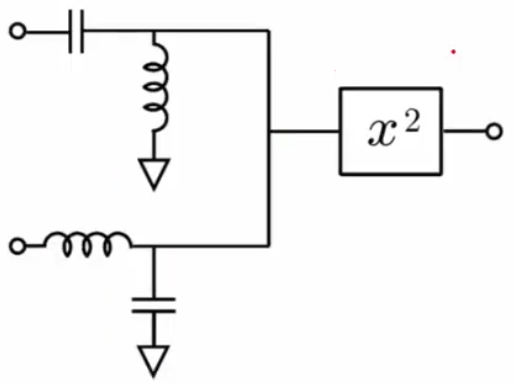
\includegraphics[width=.3\textwidth]{images/squareLaw.png}
    \label{fig:squareLaw}
    \par\vspace{0.01cm}
    {\footnotesize \raggedright Fonte: \href{https://www.youtube.com/watch?v=TaaIEdIzofc}{(RF Get Down, 2023)} \par}
\end{figure}

Para potências de entrada baixas próximas da tensão interna da junção $V_{th}$, a curva IV característica pode ser expandida em uma série de Taylor e aproximada por uma curva de ordem 2. Ao aplicarmos a soma das entrada $x_{\text{LO}} + x_{\text{RF}}$ no componente, temos a saída
\[
y(t) = a_2 \bigl( A_{\text{LO}}\cos(\omega_{\text{LO}}) + A_{\text{RF}}\cos(\omega_{\text{RF}}) \bigr)^2
\]
onde o produto pode ser expandido para gerar produtos de cossenos com as frequências $f_{\text{LO}} \pm f_{\text{RF}}$. Temos
\[
\begin{split}
y(t) = &\frac{a_2( A_{\text{LO}}^2 + A_{\text{RF}}^2)}{2} \\
& + \frac{a_2 A_{\text{LO}}^2}{2}\cos(2\omega_{\text{LO}}t) \\
& + \frac{a_2 A_{\text{RF}}^2}{2}\cos(2\omega_{\text{RF}}t) \\
& + a_2 A_{\text{LO}} A_{\text{RF}}\cos((\omega_{\text{LO}} + \omega_{\text{RF}})t) \\
& + a_2 A_{\text{LO}} A_{\text{RF}}\cos((\omega_{\text{LO}} - \omega_{\text{RF}})t)
\end{split}
\]
onde observamos a presença de produtos desejados, mas também de componentes indesejados, como o nível DC e os segundos harmônicos ($2f_{\text{LO}}$, $2f_{\text{RF}}$). Portanto o estágio final do mixer deve incluir filtros para isolar o sinal $x_{\text{IF}}$ desejado.

\section{Modelo de mixer de comutação de fase} \label{section:phaseSwitch}

As topologias que serão exploradas implementam um outro modelo de mistura a partir de comutação de fase. Neste modelo, o sinal do VCO $x_{\text{LO}}(t)$ possui potência suficientemente maior do que a tensão interna das junções $V_{th}$ para atuar como um sinal de controle, operando os componentes não-lineares como chaves ideais.

Seja $x_{\text{LO}}(t) = A_{\text{LO}}\sum_{n=1,3,\dots}^{\infty} \frac{\pi}{4n} \sin\bigl(n \omega_{\text{LO}} t\bigr)$ uma onda quadrada periódica representada em série de Fourier.

Ao realizar o produto $x_{\text{IF}}(t) = x_{\text{LO}}(t) \cdot x_{\text{RF}}(t)$ temos
\[
y(t) = A_{\text{LO}}A_{\text{RF}}\frac{\pi}{4}\cos(\omega_{\text{LO}}t)\cos(\omega_{\text{RF}}t) + A_{\text{LO}}A_{\text{RF}}\sum_{n=3,5,\dots}^{\infty} \frac{\pi}{4n} \sin\bigl(n \omega_{\text{LO}} t\bigr)
\]
onde o primeiro termo apresenta o produto desejado do modelo ideal e a soma representa demais harmônicos a serem filtrados.

Na expressão, observamos que a comutação de fase realiza cancelamento de componentes DC e harmônicos pares. Isso resulta numa perda de conversão $L_c$ menor e num espectro de saída mais limpo do que o modelo de lei quadrática.

\section{Diodo Schottky} \label{section:schottky}

O diodo Schottky é construído com uma junção metal-semicondutor, onde o semicondutor tipo P da junção P-N é substituído por um metal. A curva IV característica dos dois diodos é análoga, mas o diodo Schottky apresenta uma tensão interna da junção $V_{th}$ menor, possibilitando polarização direta para valores de voltagem aplicada $V_a$ menores do que diodos de junção P-N. Essa sensitividade permite comutação em frequências maiores do que o diodo de junção P-N e permite trabalhar com sinais de potência menor \cite{infineon}.

Para o projeto do mixer, isso também reduz a potência necessária na entrada $x_{\text{LO}}$ do VCO. Na Figura \ref{fig:schottkyIV}, extraída das especificações do diodo Schottky utilizado para o projeto, observamos $V_{th} \approx 0,51 \text{V}$.

Essa sensitividade maior do diodo Schottky pode ser explicada pelo fato de, diferentemente do diodo de junção P-N, onde a condução de corrente é feita pelos portadores minoritários em cada lado da junção (lacunas no lado N e elétrons no lado P), a condução de corrente na junção metal-semicondutor é feita por elétrons tanto no lado N quanto no lado do metal. Isso faz com que haja facilidade do fluxo de portadores (elétrons) nos dois sentidos.

Portanto, nas topologias de mixer que vamos apresentar, o diodo Schottky é preferido ao diodo de junção P-N.

\begin{figure}[h]
    \centering
    \caption{Curva IV característica para diodo Schottky SMS7621-079LF}
    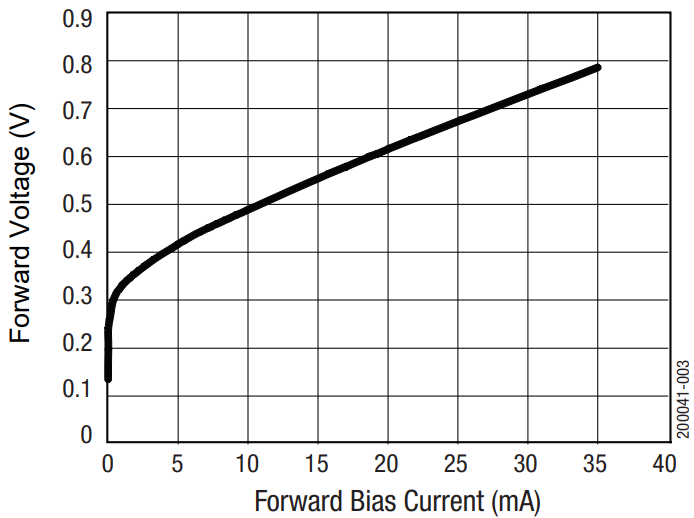
\includegraphics[width=.45\textwidth]{images/schottkyIV.png}
    \label{fig:schottkyIV}
    \par\vspace{0.01cm}
    {\footnotesize \raggedright Fonte: \cite{schottky}\par}
\end{figure}

\section{Topologias para mixers de frequência} \label{section:topologies}

Existem duas categorias principais de mixers de frequência: \textit{mixers passivos} que não requerem uma fonte de alimentação DC e são construídos utilizando diodos, e \textit{mixer ativos} com designs transistorizados que requerem alimentação DC. Nessa seção temos um apresentação de diferentes topologias estudadas (passivas e ativas) e uma análise dos prós e contras associados a cada uma. %As topologias listadas aqui foram extraídas do livro RF Electronics sugerido pelo colega da turma Andrés Hurtado  \cite{kikkert}.

\subsection{Topologia de diodo único}

A topologia de diodo único, mostrada na Figura \ref{fig:single_diode}, é muito popular em aplicações onde o custo é um fator crítico como o setor de eletrônicos de consumo onde as margens dos fabricantes são baixas.

\begin{figure}[h]
    \centering
    \caption{Mixer como topologia de diodo único para down-conversão}
    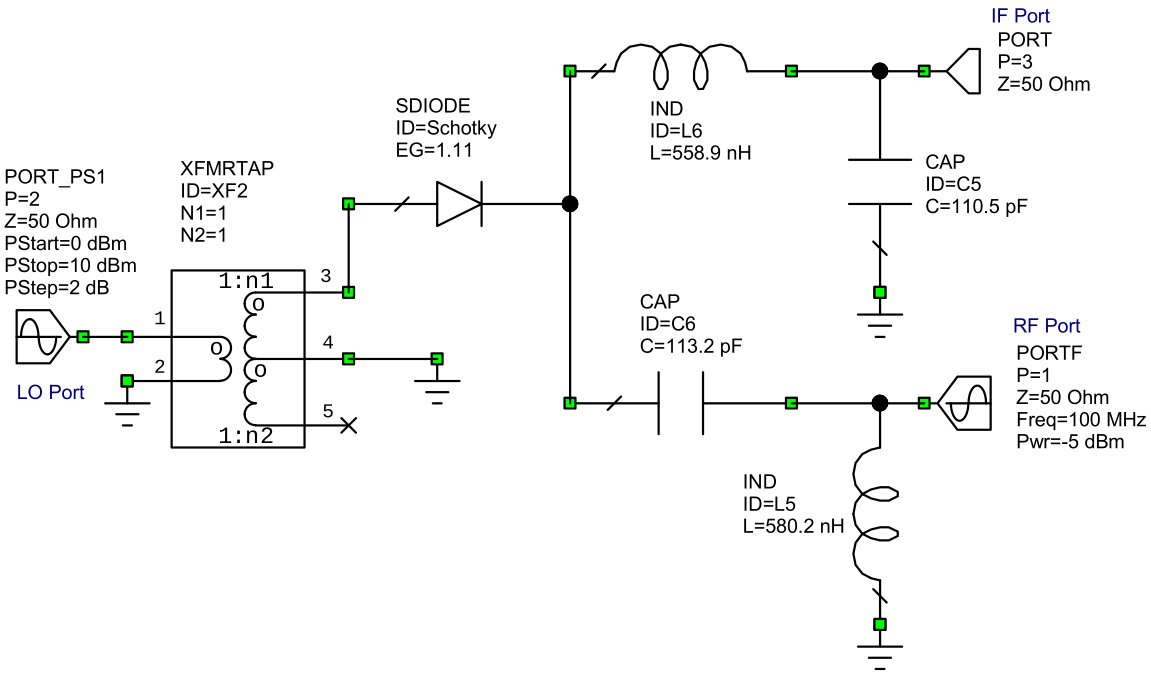
\includegraphics[width=.4\textwidth]{images/singleDiode.png}
    \label{fig:single_diode}
    \par\vspace{0.01cm}
    {\footnotesize \raggedright Fonte: \cite{kikkert}\par}
\end{figure}

Na Figura \ref{fig:single_diode}, o indutor \texttt{L5} e o capacitor \texttt{C6} ligados à entrada $x_{\text{RF}}$ atuam como um filtro passa-altas. Para frequências $\omega$ baixas, a impedância da linha
\[
Z = \frac{1}{\frac{1}{Z_{\text{RF}}} + \frac{1}{j \omega L_5}}
\]
é dominada pelo indutor em paralelo que aterra o sinal. Já para frequências $\omega$ altas, o termo $\frac{1}{j\omega L}$ vai à zero. Isso elimina ruído em frequências baixas do sinal recebido na antena RX.

Observamos que o sinal comutado pelo diodo e o sinal filtrado da antena RX são somadas na entrada de um filtro passa-baixas utilizado na saída do mixer. O capacitor \texttt{C5} nessa configuração domina a impedância da linha da saída para frequências $\omega$ altas, permitindo apenas que frequências $\omega$ baixas sejam conduzidas na saída.

\subsection{Topologia de par de diodos}

Um componente que salta aos olhos na topologia de par de diodos, mostrada na Figura \ref{fig:two_diodes}, é o acoplador de anel híbrido (em inglês, também chamado de rat-race) aplicado sobre as entradas do par de diodos que é responsável pelo casamento de impedância para otimizar a transferência de potência e pela mistura dos sinais \cite{ratrace}.

\begin{figure}[h]
    \centering
    \caption{Mixer como topologia de par de diodos para down-conversão}
    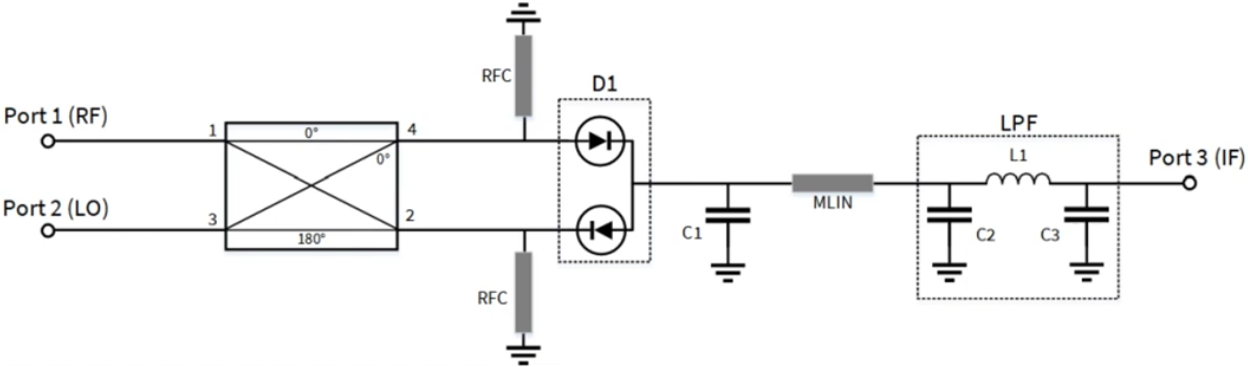
\includegraphics[width=.45\textwidth]{images/twoDiodes.png}
    \label{fig:two_diodes}
    \par\vspace{0.01cm}
    {\footnotesize \raggedright Fonte: \cite{infineon}\par}
\end{figure}

Diferente da soma de sinais feita no diplexer, a geometria do anel faz com que a potência de RF seja distribuída em fase ($0^\circ$) para ambos os diodos Schottky, enquanto o sinal do oscilador local (LO) é entregue com uma defasagem de $180^\circ$ entre os dois ramos. Essa alimentação em oposição de fase garante que o ruído de amplitude no VCO seja cancelado por interferência destrutiva no nó de saída, resultando mais limpo na saída $x_{\text{IF}}$. Além do cancelamento de ruído, a simetria do acoplador oferece um bom isolamento entre as portas LO e RF, impedindo que o sinal de alta potência do VCO vaze para a antena de recepção e degrade a sensibilidade do sistema.

Observamos que os indutores de RF choke em paralelo com os diodos, indicados na Figura \ref{fig:two_diodes} com a sigla RFC \cite{RFchoke}, atuam como filtros passa-baixas, dimensionados para bloquear altas frequências na entrada dos diodos.

\subsection{Topologia de anel de diodos}

A topologia clássica para mixer ativos é a topologia de anel de diodos, mostrada na Figura \cite{ADI_Ch4}.

\begin{figure}[h]
    \centering
    \caption{Mixer com a topologia passiva de anel de diodos}
    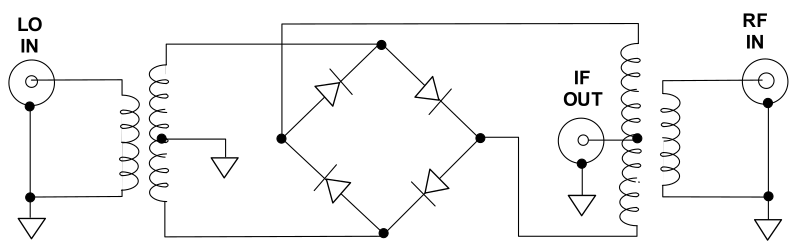
\includegraphics[width=.4\textwidth]{images/diode_ring_mixer.png}
    \label{fig:diode_ring}
    \par\vspace{0.01cm}
    {\footnotesize \raggedright Fonte: \cite{ADI_Ch4}\par}
\end{figure}

Na Figura \ref{fig:diode_ring}, observamos que as duas entradas são decompostas em entradas diferenciais com defasagem de $180^\circ$
\begin{align*}
    \begin{cases}
        x_{\text{LO}}(t) &= x_{\text{LO}+}(t) + x_{\text{LO}-}(t) \\
        x_{\text{RF}}(t) &= x_{\text{RF}+}(t) + x_{\text{RF}-}(t)
    \end{cases}
\end{align*}
e os pares dessas entradas diferenciais definem a polarização dos diodos no anel e comutam o sinal que é transmitido para a saída $x_{\text{IF}}(t)$.

\subsection{Topologia célula de Gilbert}

Nessa seção, apresentamos um exemplo de topologia ativa: a célula de Gilbert, mostrada na Figura \ref{fig:gilbert}.

Enquanto nas topologias passivas a comutação de sinais pelos diodos Schottky era feita em tensão, a célula de Gilbert comuta os sinais de entrada em corrente. Na Figura \ref{fig:gilbert}, vemos que um bloco fundamental na célula de Gilbert é o par diferencial CMOS que implementa os estágio de transcondutância e comutação do circuito.

\begin{figure}[h]
    \centering
    \caption{Mixer com a topologia ativa de célula de Gilbert}
    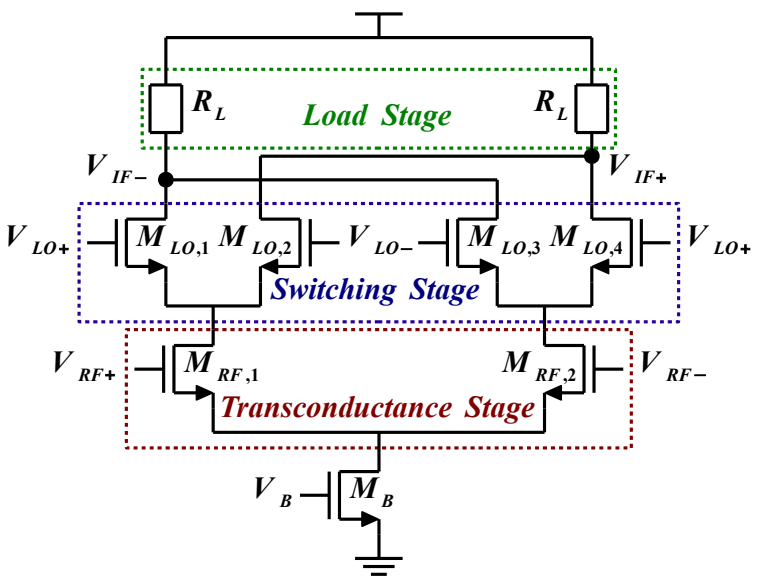
\includegraphics[width=.4\textwidth]{images/gilbertCell.png}
    \label{fig:gilbert}
    \par\vspace{0.01cm}
    {\footnotesize \raggedright Fonte: \cite{vivas2014}\par}
\end{figure}

Para compreender o funcionamento da célula, analisamos primeiro o ponto de operação DC de um par diferencial isolado, mostrado na Figura \ref{fig:diffPair}. Para isso, suponha que ambas as entradas estejam aterradas. Temos

\begin{align}
		I_{D_1} + I_{D_2} &= I_Q \\
		I_{D_1} &= I_{D_2} \quad \text{ por simetria}
\end{align}

A corrente de dreno é fixada pela fonte de corrente supondo que ambos os transistores estejam na saturação, as tensões de fonte se estabilizarão em um valor que satisfaça $I_{D_1} = I_{D_2} = \frac{I_Q}{2}$.

Uma variação nas entradas tal que $V_{G_1} > V_{G_2}$ causa um desequilíbrio de modo que $V_{GS_1}$ torna-se maior que $V_{GS_2}$, fazendo com que $I_{D_1}$ aumente e, consequentemente, $I_{D_2}$ diminua.

\begin{figure}[h]
    \centering
    \caption{Circuito do par diferencial}
    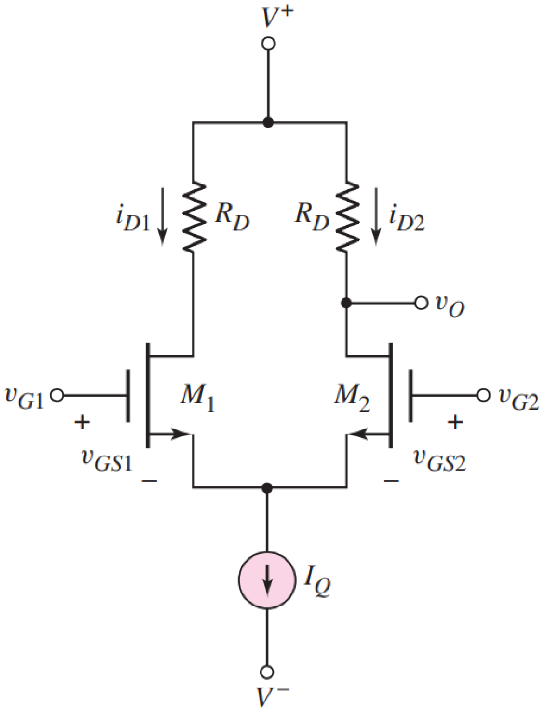
\includegraphics[width=.3\textwidth]{images/diffPair.png}
    \label{fig:diffPair}
    \par\vspace{0.01cm}
    {\footnotesize \raggedright Fonte: \cite{neaman}\par}
\end{figure}

Dessa forma, na célula de Gilbert, o par diferencial no estágio de transcondutância converte o sinal de radiofrequência $V_{RF}$ em variações de corrente para os estágios superiores.

No estágio de comutação, quando o semiciclo da entrada $x_{\text{LO}}$  do VCO é positivo ($V_{\text{LO}+} > V_{\text{LO}-}$), a corrente flui preferencialmente por um braço do par, e quando o semiciclo é negativo ($V_{\text{LO}-} > V_{\text{LO}+}$), a corrente é direcionada para o braço oposto. As impedâncias no topo da célula convertem as correntes comutadas de volta para tensões $V_{\text{IF}-}$, $V_{\text{IF}+}$ representando as saídas do mixer nas frequências $f_{\text{LO}} \pm f_{\text{RF}}$.

\section{Design e simulação no ADS} \label{section:ADS}

Optamos por uma topologia passiva para simplificar o design do mixer uma vez que não precisamos nos preocupar com a alimentação no caso dos diodos. A construção do circuito passivo com diodos também se revelou mais barata quando procuramos por componentes no site da Mouser. Entre as topologias passivas, a topologia escolhida foi a de par de diodos Schottky por fornecer um bom compromisso entre isolamento, baixa perda de conversão e complexidade do design.

\subsection{Design do acoplador de anel híbrido}

\textcolor{red}{futuro...}

\subsection{Design do mixer com par de diodos}

\textcolor{red}{futuro...}

\newpage
\bibliography{refs}
\bibliographystyle{icml2024}

\end{document}